\chapter{Multiple Hypothesis testing, Covariance, Correlation}

\section{The Bonferroni correction}
When performing statistical test, we often want to use the same data
set to test many different alternative hypotheses. For example, when
studying high blood pressure we might want to support or refute
the following hypotheses
\begin{enumerate}
\item Blood pressure is elevated in patients with high cholesterol.
\item Blood pressure is elevated in older patients.
\item High blood pressure is caused by stress.
\item Blood pressure is elevated in patients that eat too many
  vegetables.
\item and so on.
\end{enumerate}
Suppose we run a test whose significance is $\alpha$ for each of these
hypotheses and find that one of the tests rejects the null
hypothesis. Can we say that the significance of this rejection is
$\alpha$? Clearly, as the number of tests increases, the significance
of each test decreases. How can we account for that? It is tempting to
think of passing each test as an independent event and calculate the
overall significance based on that. However, we don't know whether the
tests are independent or not. In fact, the opposite is probably true:
older patients tend to also have high cholesterol.

We therefor do the safe thing and use the union bound. Let $T_i$,
$i=1,\ldots,n$ be the event corresponding to test $i$ rejecting the
null hypothesis when the null hypothesis is in fact true. Suppose that
the $p$ value of each of the $n$ tests is at most $\alpha$,
i.e. $P(T_i) \leq \alpha$.
 
The union bound tells us that 
\[
P\left( \bigcup_{i=1}^n T_i \right) \leq \sum_{i=1}^n P(T_i) \leq n \alpha
\]

\section{Catch, mark and release}
Statistical techniques are useful for estimating the size of a large
population. Suppose for example that we want to count the number of
fish in a lake. How would we do that? Instead of trying to catch all
the fish, which is both impossible and damaging to the fish
population, we perform the following two phase test:
\begin{enumerate}
\item We catch fish, mark them with some non-intrusive marker, and
  release them back to the lake. Suppose we mark $m$ of them with a
  mark that sticks to the fish but does not hurt it.
\item After we marked the $m$ fish, we wait for them to mix with the
  other fish and then catch $l$ fish and count how many of these
  have been marked. We denote the number of marked fish by the random
  variable $Y$.
\end{enumerate}
The probability that each that each fish caught in the second batch is
marked is equal to the fraction of all of the fish in the lake that
are marked, which is $m/n$. This means that the random variable $Y$ is
a sum of $l$ independent binary random variables each with mean $m/n$.
Therefor the mean of $Y$ is $(lm)/n$. The standard deviation of each
of the binary variables is at most $1/2$ (which happens when
$m/n=1/2$). Thus the standard deviation of $Y$ is $\sqrt{l}/2$.
Therefor the 95\% significance interval for $(lm)/n$ is
$[Y-\sqrt{l},Y+\sqrt{l}]$.

We are interested in estimating $n$, therefor our estimate is the range.
\[
\left[\frac{lm}{Y+\sqrt{l}}, \frac{lm}{Y-\sqrt{l}} \right]
\]

Note that if the number of fish in the lake $n$ is large, so that $m/n
\approx 1/l$ then there is a good chance we will see no marked fish in
the second batch. We might need to mark more and more fish until the
chance of catching a marked fish becomes reasonably high.

\section{Covariance}

Two random variables $X,Y$ are independent if and only if for any
constants $a,b$
we have:
\[
P(X\leq a \text{ and } Y \leq b)=P(X\leq a)P(Y \leq b)
\]
If $X,Y$ are restricted to the integers, then they are independent if
and only if for any two integers $i,j$
\begin{equation} \label{eqn:independentRVs}
P(X=i \text{ and } Y=j)=P(X=i)P(Y=j)
\end{equation}
Suppose we further restrict $X,Y$ to the integers $1,\ldots,100$. In
order to check whether or not $X$ and $Y$ are dependent we need to
check $100^2=10000$ conditions. Checking for independence of these random
variables requires estimating 10,000 joint probabilities, which in
turn requires very large samples.

There is an easy to calculate stand-in for dependence, called
the {\em covariance}, which we will now describe. If the covariance is not
zero then the two random variables are dependent. However, a
covariance of zero between two random variables {\em does not} imply
that they are independent.

The covariance of $X$ and $Y$ is defined as
\[
Cov(X,Y) = E\left[ (X-E(X))(Y-E(Y)) \right]
\]
Note that $Cov(X,X)=Var(X)$. We can simplify the expression for the
covariance as follows:
\[
E\left[ (X-E(X))(Y-E(Y)) \right]
=E[XY]-E[E[X]Y]-E[XE[Y]]+E[X]E[Y]
=E[XY] -E[X]E[Y]
\]
We will now show that if $X$ and $Y$ are independent then the
covariance is zero. We will show this for integer valued random
variables~\footnote{The extension to continuous random variables is
  straight forward, but involves some technical issues involving
  integration that we will not get into here.}
\begin{eqnarray}
E[XY]&=&\sum_{i,j} ij P(X=i \text{ and } Y=j) \label{EXY:1}\\ 
&=& \sum_{i,j} ij P(X=i)P(Y=j) \label{EXY:2}\\
&=& \left( \sum_i i P(X=i) \right)\left( \sum_j j P(Y=j) \right)\label{EXY:3}\\
&=&E[X]E[Y] \label{EXY:4}
\end{eqnarray}
Equation~(\ref{EXY:1}) follows from the definition of expectation
($i,j$ vary from $-\infty$ to $+\infty$). Equation~(\ref{EXY:2})
follows from Equation~(\ref{eqn:independentRVs}). We separate the
double summation in Equation~(\ref{EXY:2}) into a product of two sums
to get Equation~(\ref{EXY:3}), and finally use the definition of
expectation to get Equation~(\ref{EXY:4}). Thus we have shown that
when two random variables $X,Y$ are independent, then $E[XY]=E[X]E[Y]$
and thus $Cov(X,Y)=E[XY]-E[X]E[Y]=0$.

Intuitively, $Cov(X,Y)>0$ indicates that when $X$ is large $Y$ also
tends to be large. When this happens we say that $X$ and $Y$ are {\em
  correlated}. If $Cov(X,Y)<0$ we say that $X$ and $Y$ are {\em
  anti-correlated}, and if $Cov(X,Y)=0$. We say that $X$ and $Y$ are
{\em uncorrelated}. 

One problem with the covariance is it's sensitivity to the units in
which the random variables are measured, changing the scale changes
the covariance. Suppose the sample space corresponds to people and
suppose we consider two random variables for each person: $H$ is the
height of the person, in inches, and $W$ is the weight of the person,
in pounds.  We expect the the $H$ and $W$ are correlated. However, how
should we measure the {\em degree} of correlation? $Cov(H,W)$ will
decrease if we decide to use feet instead of inches because that would 
decrease each height by a factor of 12 and we get
$Cov(H/12,W)=Cov(H,W)/12$. In order to remove the effect of scale we
use a normalized version of the covariance, called the correlation
coefficient:
\[
Corr(X,Y) \doteq \frac{Cov(X,Y)}{\sqrt{Var(X)Var(Y)}}
\]
The correlation coefficient is a number in the range $[-1,1]$. As with
the Covariance, if $Corr(X,Y)>0$ we say that $X$ and $Y$ are {\em
  correlated}, if $Corr(X,Y)=0$ we say that $X$ and $Y$ are {\em
  uncorrelated} and if $Corr(X,Y)<0$ we say that $X$ and $Y$ are {\em
  anti-correlated}.

The extreme cases are interesting. If $Corr(X,Y)=1$ it means that
$X=aY$ for some $a>0$ while if $Corr(X,Y)=-1$, $X=aY$ for some
$a<0$. These and other interesting cases are depicted in Figure~\ref{fig:corrCoeff}.

\begin{figure}[tb]
\begin{center}
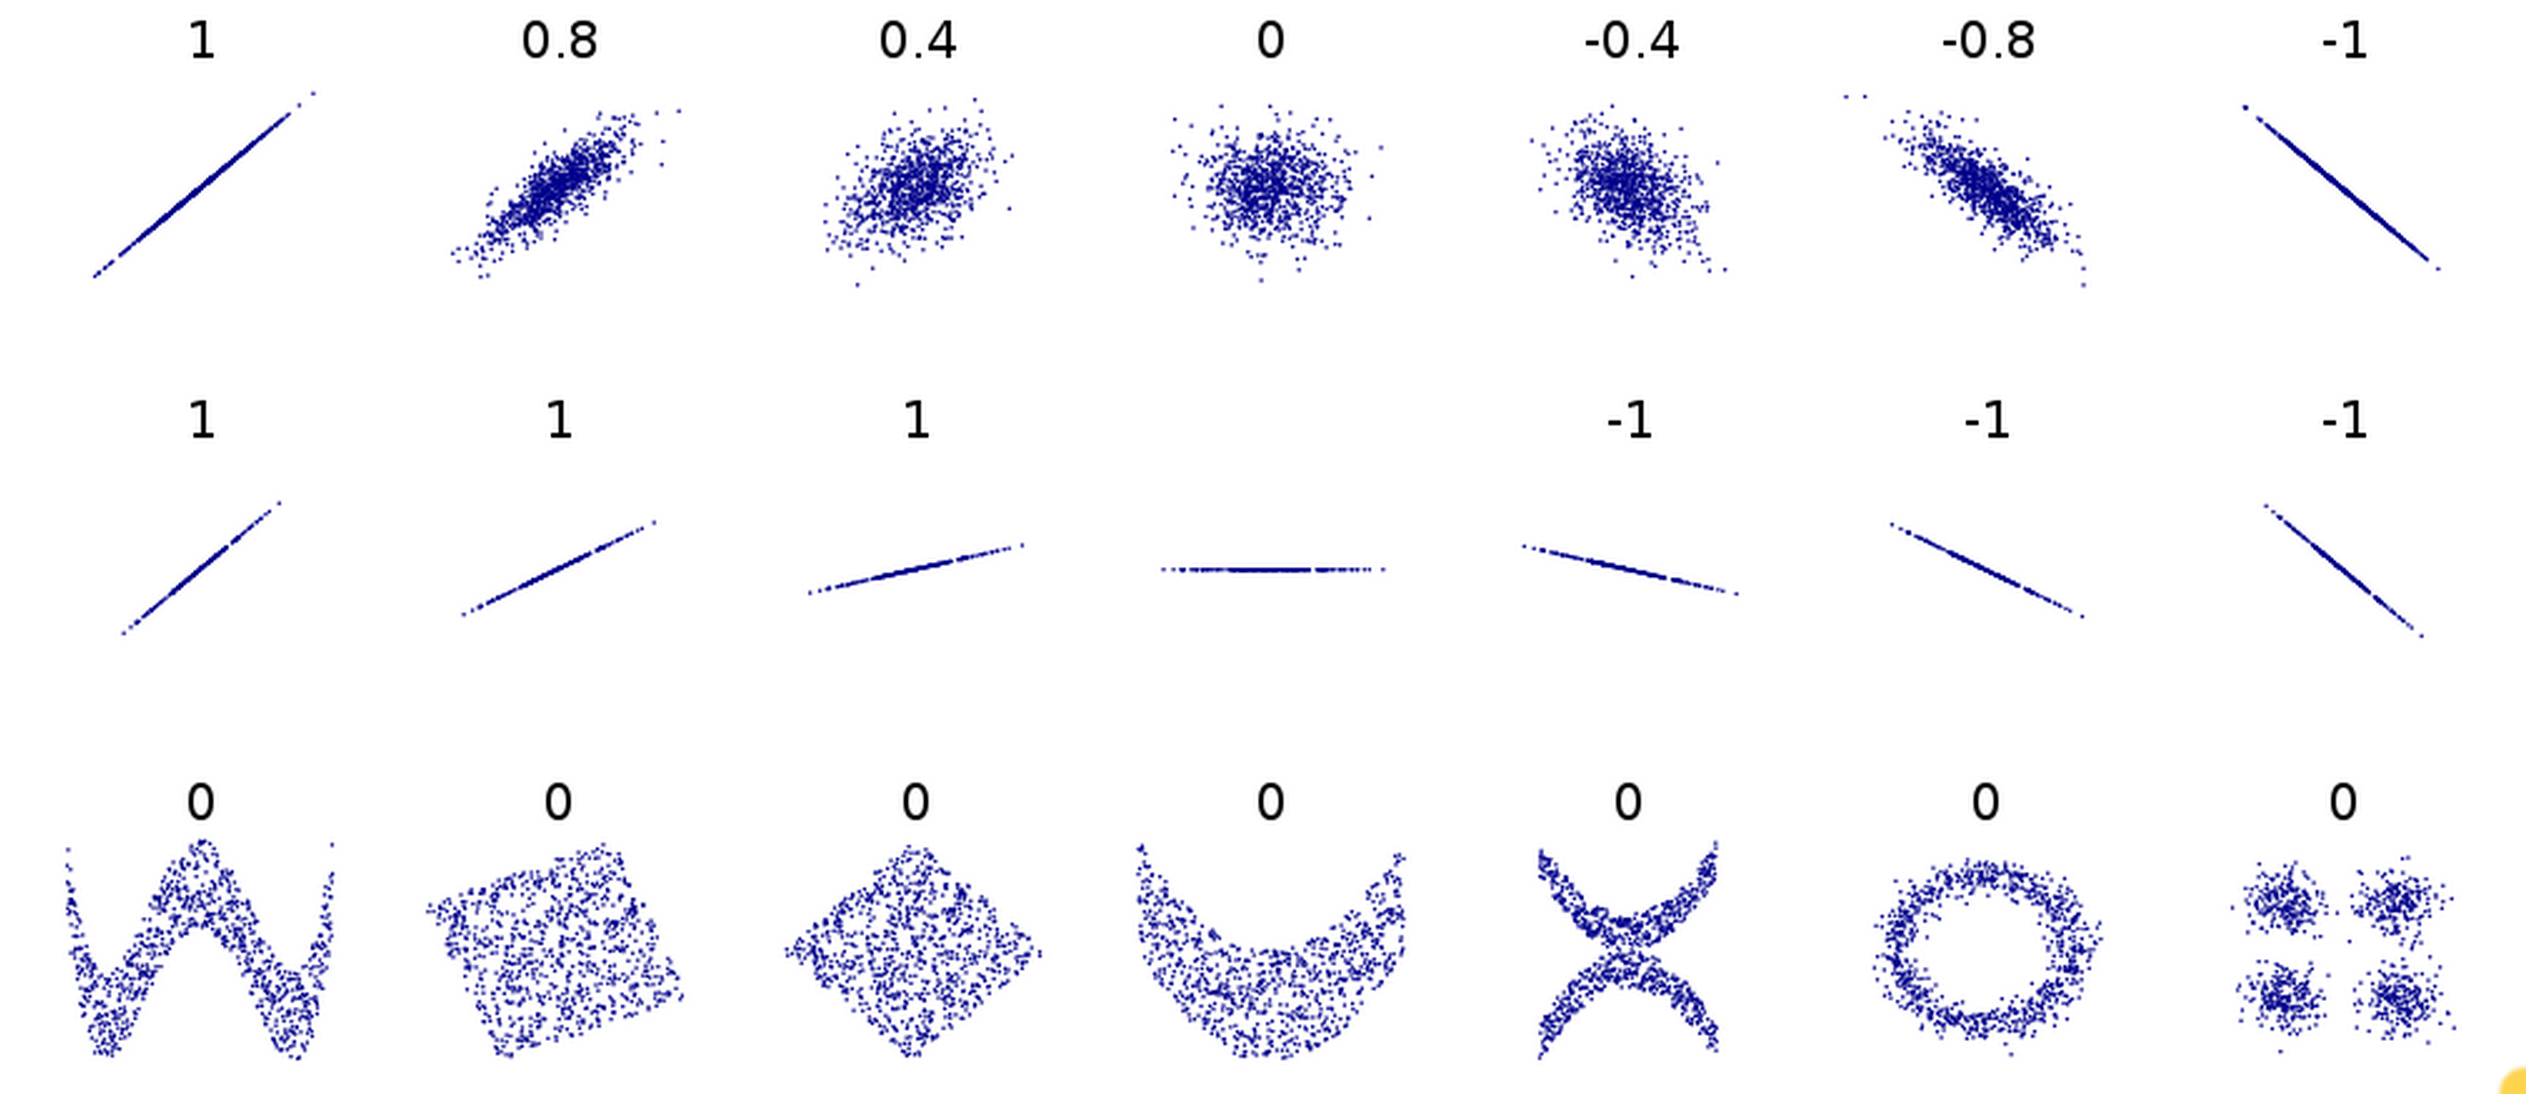
\includegraphics[width=5in]{figs/correlationCoefficients.png}
\end{center}
\caption{\label{fig:corrCoeff} Examples of joint distributions and
  their corresponding correlation coefficients. The distributions are
  represented by a sample of points drawn IID from the underlying
  distribution. The number next to each cloud of points is the value 
  of the correlation coefficients corresponding to the distribution. 
{\bf The top row} shows ellipsoidal distributions with varying levels of
correlation. {\bf The middle row} shows distributions that are concentrated
on a line of the form $X=aY$, the correlation for these distributions
is one of $-1,0,+1$ depending on the value of $a$. {\bf The bottom
  row} shows a variety of distributions where $X$ and $Y$ are
uncorrelated. These distributions demonstrate some of the many ways in
which uncorrelated random variables can be dependent.(Image taken from
WikiPedia:Correlation Coefficients)}
\end{figure}

An example of correlated random variables are the
price of fuel and the price of food. In this case there is a
direct cause and effect: fuel prices influence food prices because
manufacturing and distributing food requires large amounts of fuel. In
general, there might not be a causal relationship between two
correlated random variable. For example, consider the sentence: ``As
ice cream sales increase, the rate of drowning deaths increases
sharply. Therefore, ice cream causes drowning.''. The factual part of
the sentence is that there is a correlation between the random
variables corresponding to ``ice-cream sales'' and ``the rate of
drowning deaths''. However, the correlation does not imply
causation. The probable common cause for increases in both ice cream sales and
drowning deaths is increases in the number of people that come to the beach.  A
reminder against making this mistake is the statistical dictum
{\em ``Correlation does not imply causation''}

However, correlation {\em does} imply dependence because, as we show,
independence implies that the covariance is zero. The opposite
direction does not hold, in other words, zero covariance does not
imply that the two random variables are independent. Here is a simple
example, $X$ and $Y$ attain the values $-1,0,1$ but only the following
four combinations have non-zero probability. Specifically
\[
P(X=-1 \wedge Y=0)=
P(X=+1 \wedge Y=0)=
P(X=0 \wedge Y=-1)=
P(X=0 \wedge Y=+1)=1/4
\]
(where $\wedge$ correspond to ``and''). On the one hand, it is easy to
see that the covariance is zero, because the expected values of $X$,
$Y$ and $XY$ are all zero. On the other hand, $X$ and $Y$ are not
independent because $P(X=0 \wedge Y=0)=0$ while $P(X=0)=1/2$ and
$P(Y=0)=1/2$, and thus $P(X=0 \wedge Y=0) \neq P(X=0)P(Y=0)$

